\documentclass[compress, red]{beamer}

\usepackage[utf8]{inputenc}
\usepackage{xcolor}
\usepackage{listings}


\definecolor{bordeaux}{rgb}{178, 51, 51}

\usetheme{Warsaw}

%------------------------------------------------------------
%This block of code defines the information to appear in the
%Title page
\title[Projet HAX712X] %optional
{Projet HAX712X METH}

\subtitle{Prédiction et visualization de la consommation d'électricité en France}

\author[M. Akkouh, E. Cerezo, T. Laugié, H. Slama] % (optional)
{Maryam Akkouh \and Ema Cerezo\\ Thomas Laugié \and Hamza Slama}


\date[VLC 2021] % (optional)
{Rapport de mi-projet, décembre 2022}

\logo{
\includegraphics[height=1cm]{images/logo-ssd.png}}

%End of title page configuration block
%------------------------------------------------------------

%------------------------------------------------------------
%The next block of commands puts the table of contents at the 
%beginning of each section and highlights the current section:

\AtBeginSection[]
{
  \begin{frame}
    \frametitle{Table of Contents}
    \tableofcontents[currentsection]
  \end{frame}
}

%------------------------------------------------------------

\begin{document}

%The next statement creates the title page.
\frame{\titlepage}

%---------------------------------------------------------
%This block of code is for the table of contents after
%the title page
\begin{frame}
\frametitle{Table of Contents}
\tableofcontents
\end{frame}
%---------------------------------------------------------


\section{Introduction}
\begin{frame}
\begin{figure}[h!]
	\begin{minipage}[b]{0.01\linewidth}
	  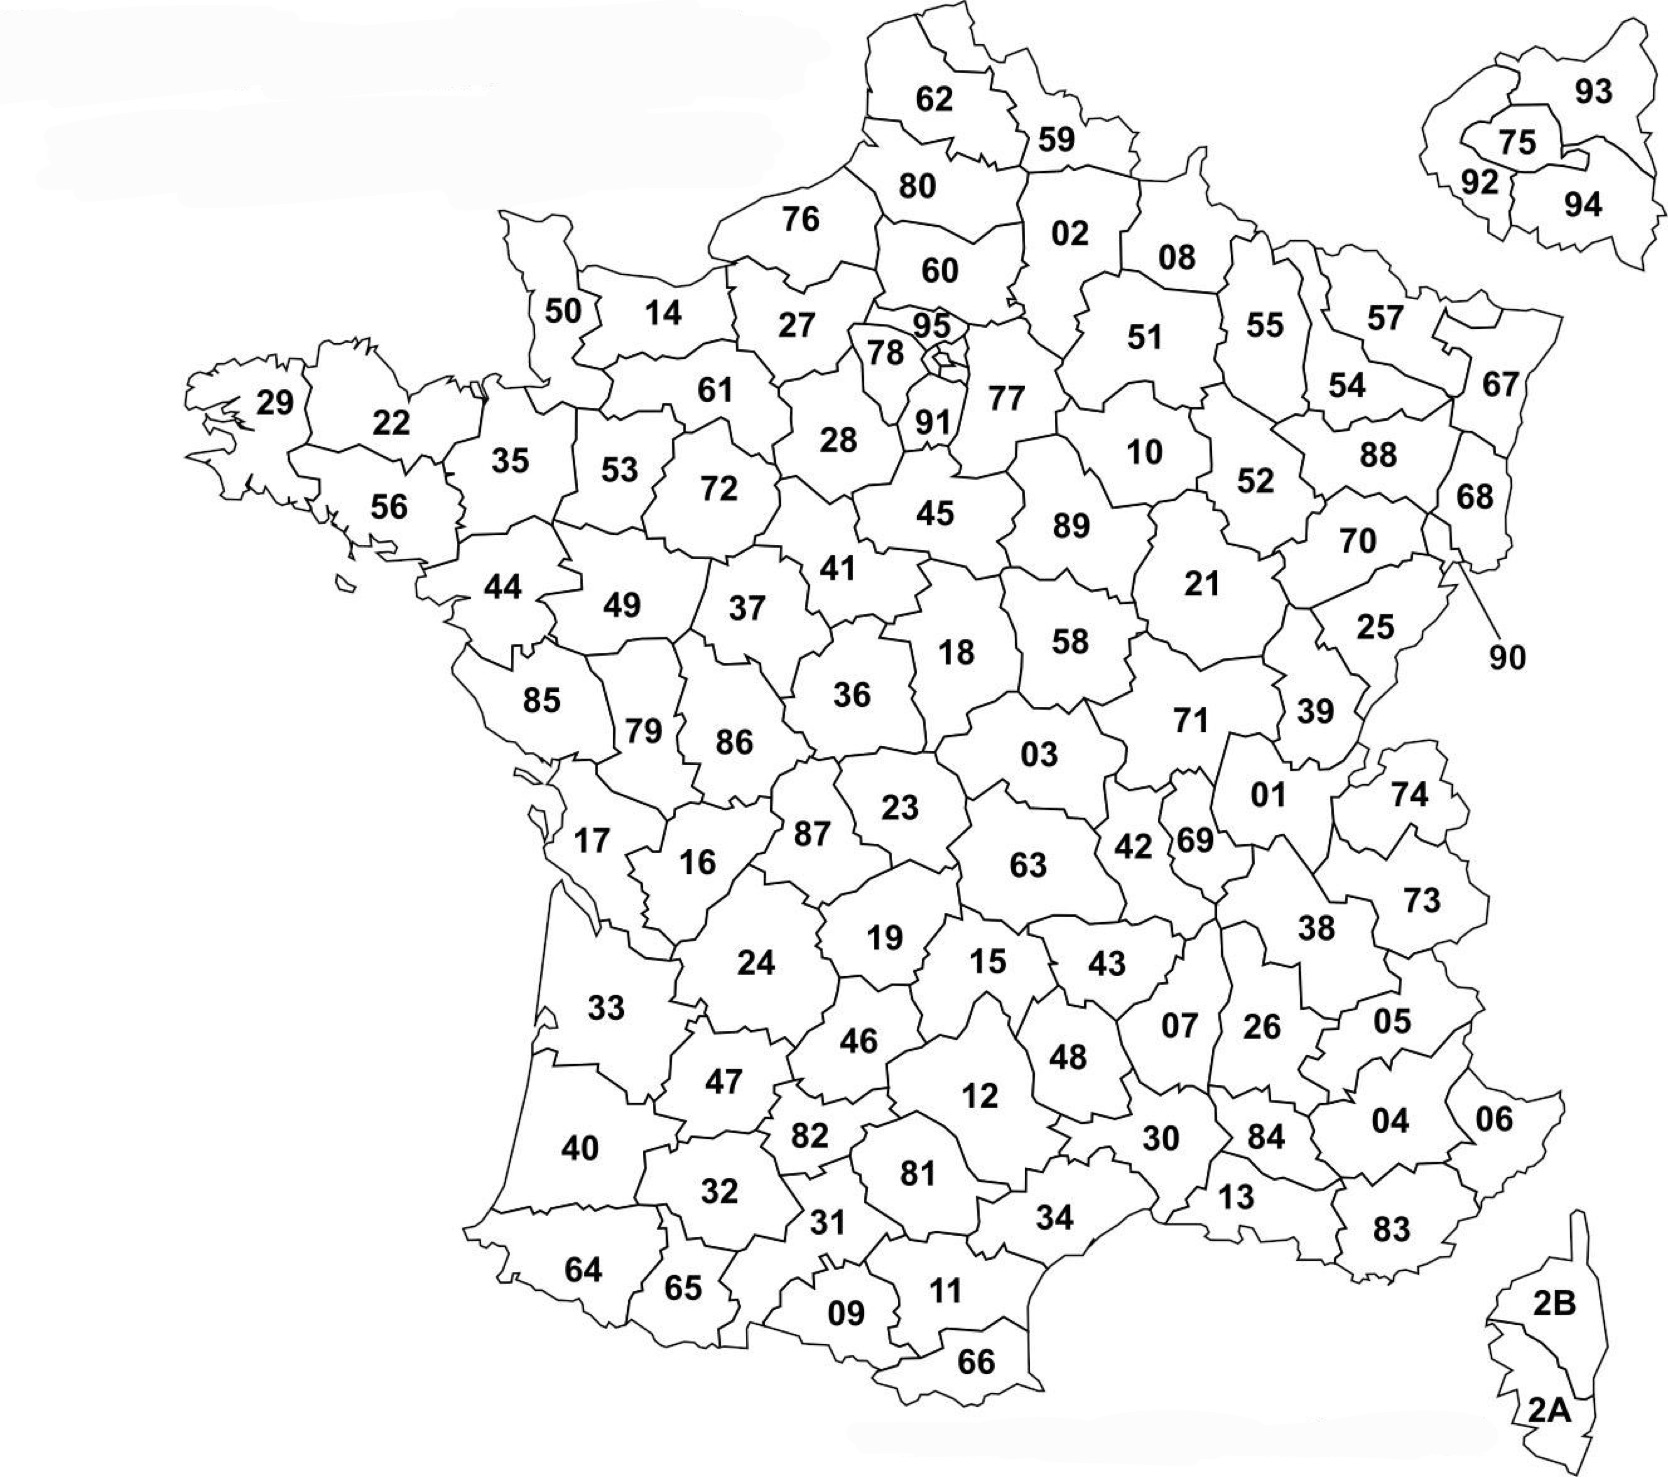
\includegraphics[scale=0.1]{images/Image (1)-1.jpg}
	\end{minipage}\hfill
	\begin{minipage}[b]{0.4\linewidth}	
		\centering 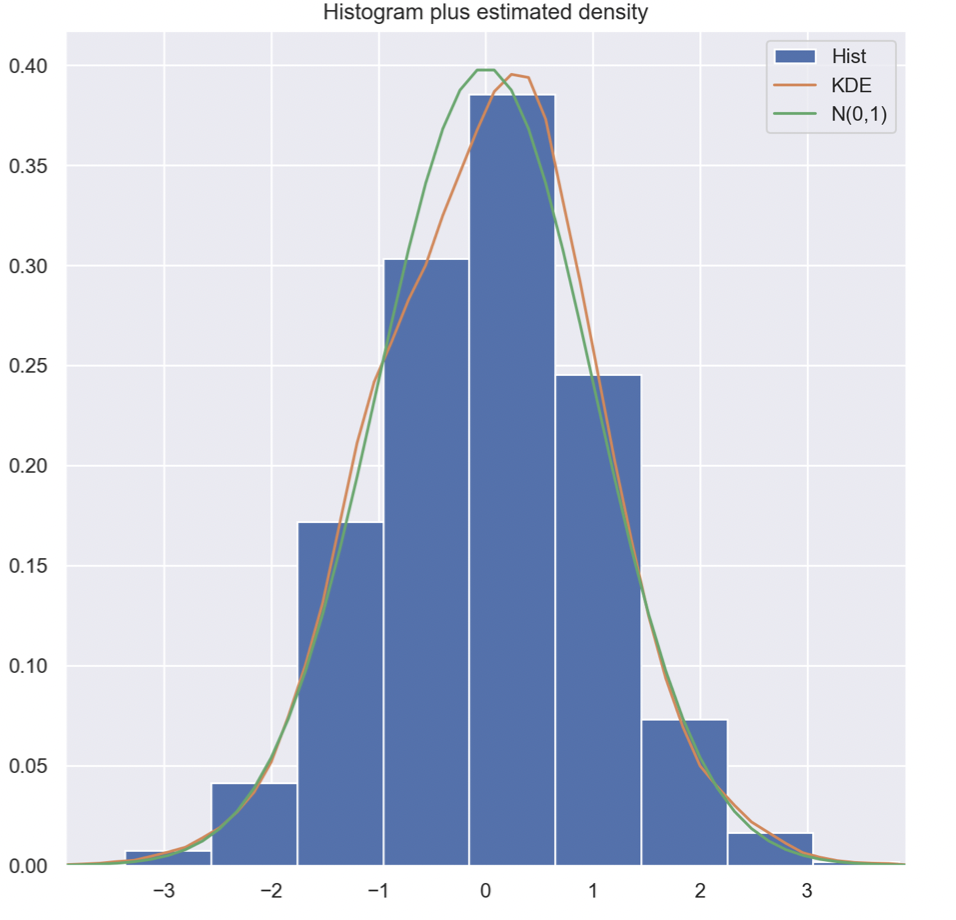
\includegraphics[scale=0.3]{images/histogramme.png}
	\end{minipage}
\end{figure}
\end{frame}



\section{Traitement des données}

%---------------------------------------------------------
%Highlighting text
\begin{frame}
\frametitle{Traitement des données}


\begin{block}{Nettoyage des données}
Enlever le informations inutiles
\end{block}

\begin{block}{Création de foncions}
Extraction des données pour les rendre utilisable
\end{block}


\end{frame}
%---------------------------------------------------------


\begin{frame}
\frametitle{Exemple}
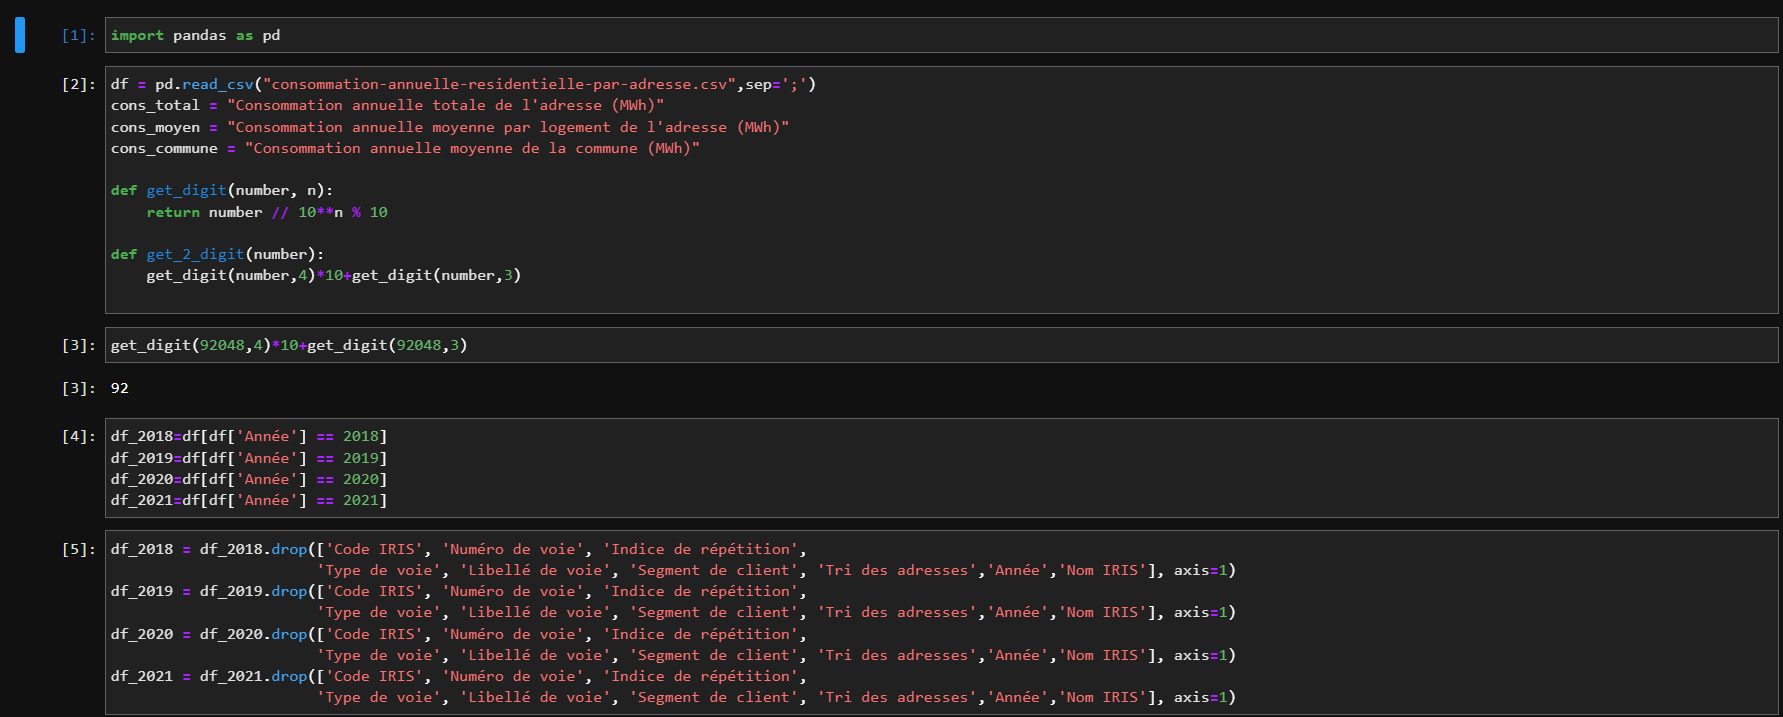
\includegraphics[scale=0.30]{images/Imagedonnee.png}

\end{frame}


\section{Visualisation}

%---------------------------------------------------------
%Highlighting text
\begin{frame}
\frametitle{Données utilisées et packages principaux}

Données :
\begin{itemize}
\item Enedis
\item France-geojson
\end{itemize}

\vspace{0.5cm}

Packages :
\begin{itemize}
\item Pandas, geopandas 
\item Folium
\item Streamlit
\end{itemize}

\vspace{0.5cm}

Référence :
\begin{itemize}
\item Streamlit-map-dashboard
\end{itemize}

\end{frame}
%---------------------------------------------------------


%---------------------------------------------------------
%Two columns
\begin{frame}
\frametitle{Rendu}

\vspace{-0.5cm}

\begin{center}
    \fbox{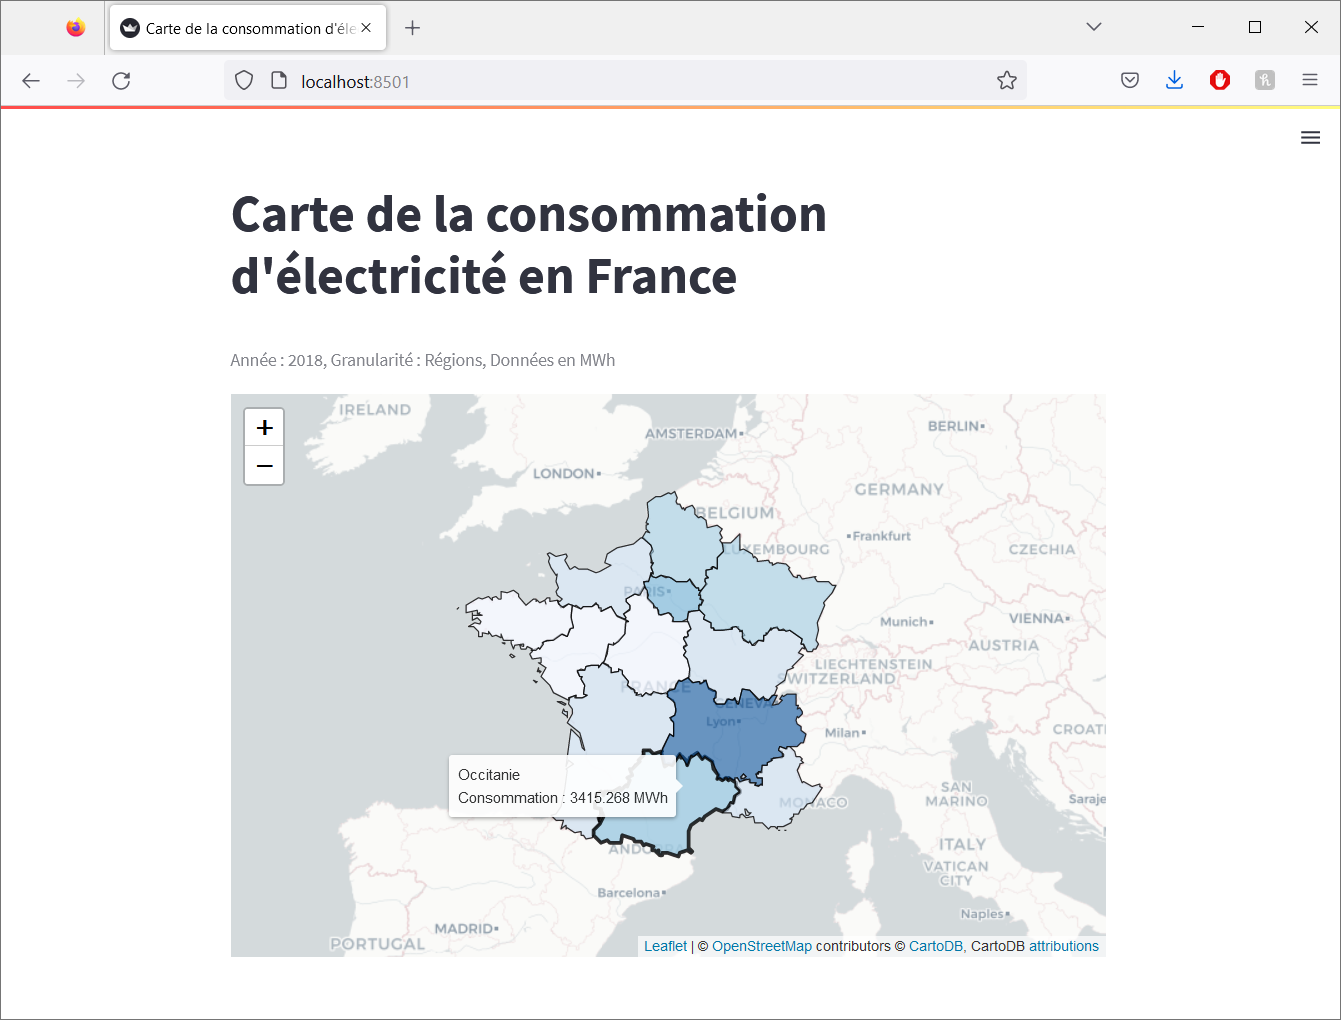
\includegraphics[scale=0.3]{images/Carte_DevLog.png}}
\end{center}

\end{frame}
%---------------------------------------------------------



\section{Prédictions}

%---------------------------------------------------------
%Highlighting text
\begin{frame}{Création de base des données }
\begin{center}
\begin{overprint}
\only<1>{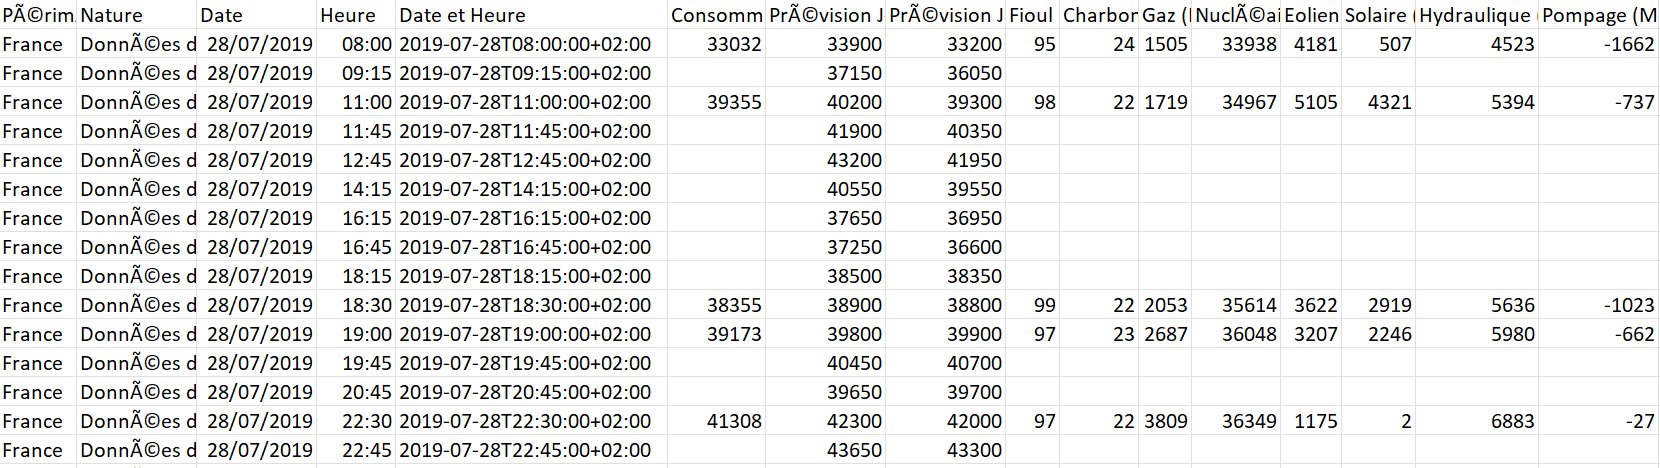
\includegraphics[scale=0.40]{images/imagedata1.png}}
\hspace{-0.17em}\only<2>{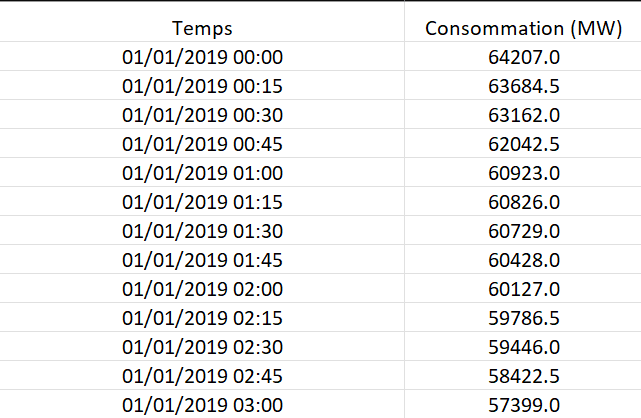
\includegraphics[scale=0.40]{images/imagedata2.png}}
\only<1>{\mbox{\structure{Figure:} data originale }}

\only<2>{\mbox{\structure{Figure:} data finale}}

\end{overprint}
\end{center}
\end{frame}
%---------------------------------------------------------


%---------------------------------------------------------
%Two columns
\begin{frame}
\frametitle{Modèle de prédiction UCM}
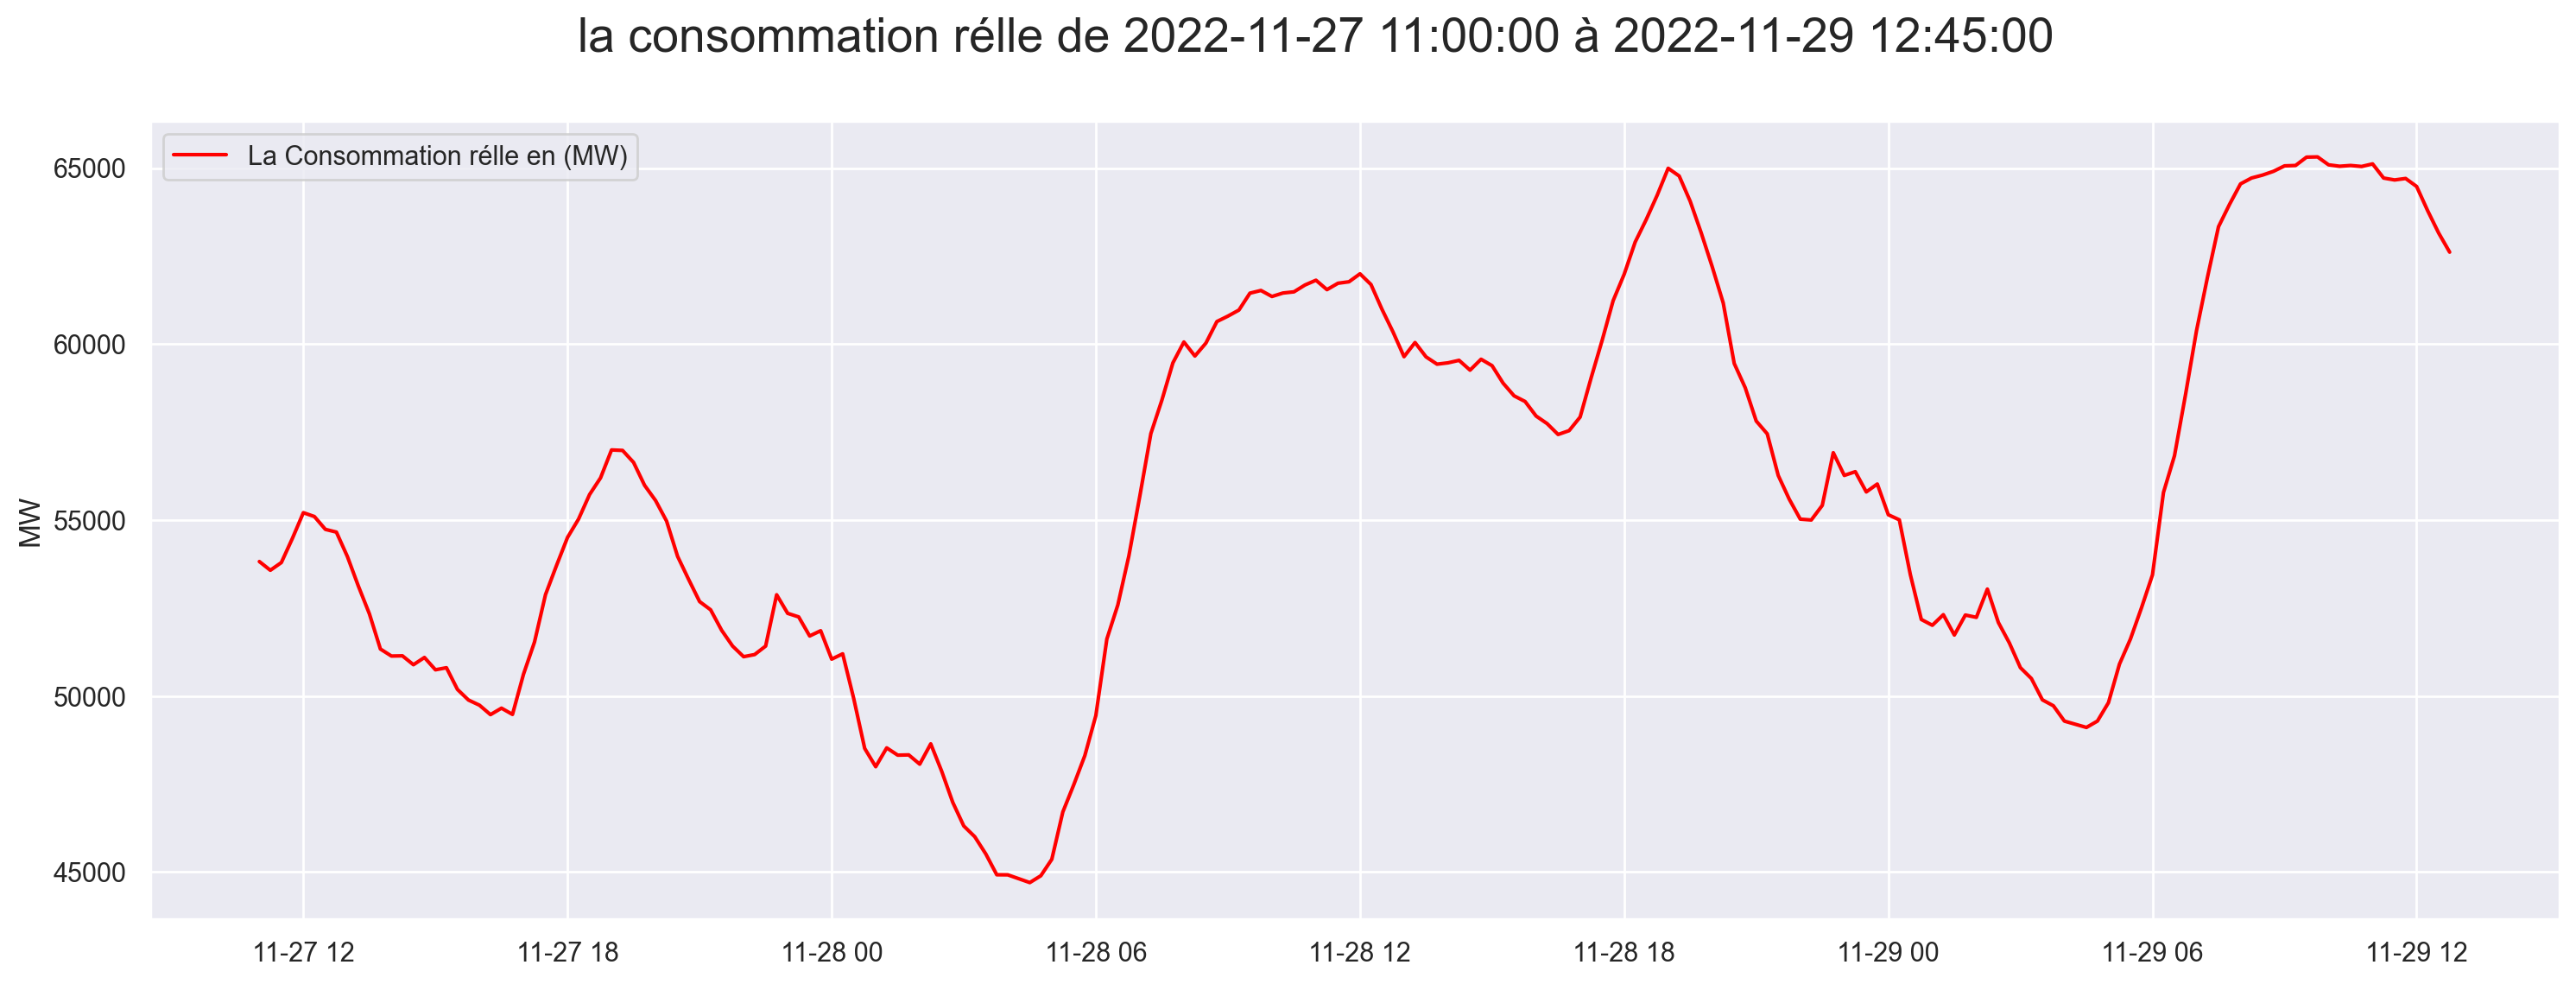
\includegraphics[scale=0.30]{images/outputR.png}

\end{frame}
%---------------------------------------------------------


%---------------------------------------------------------
%Two columns
\begin{frame}
\frametitle{Modèle de prédiction UCM}
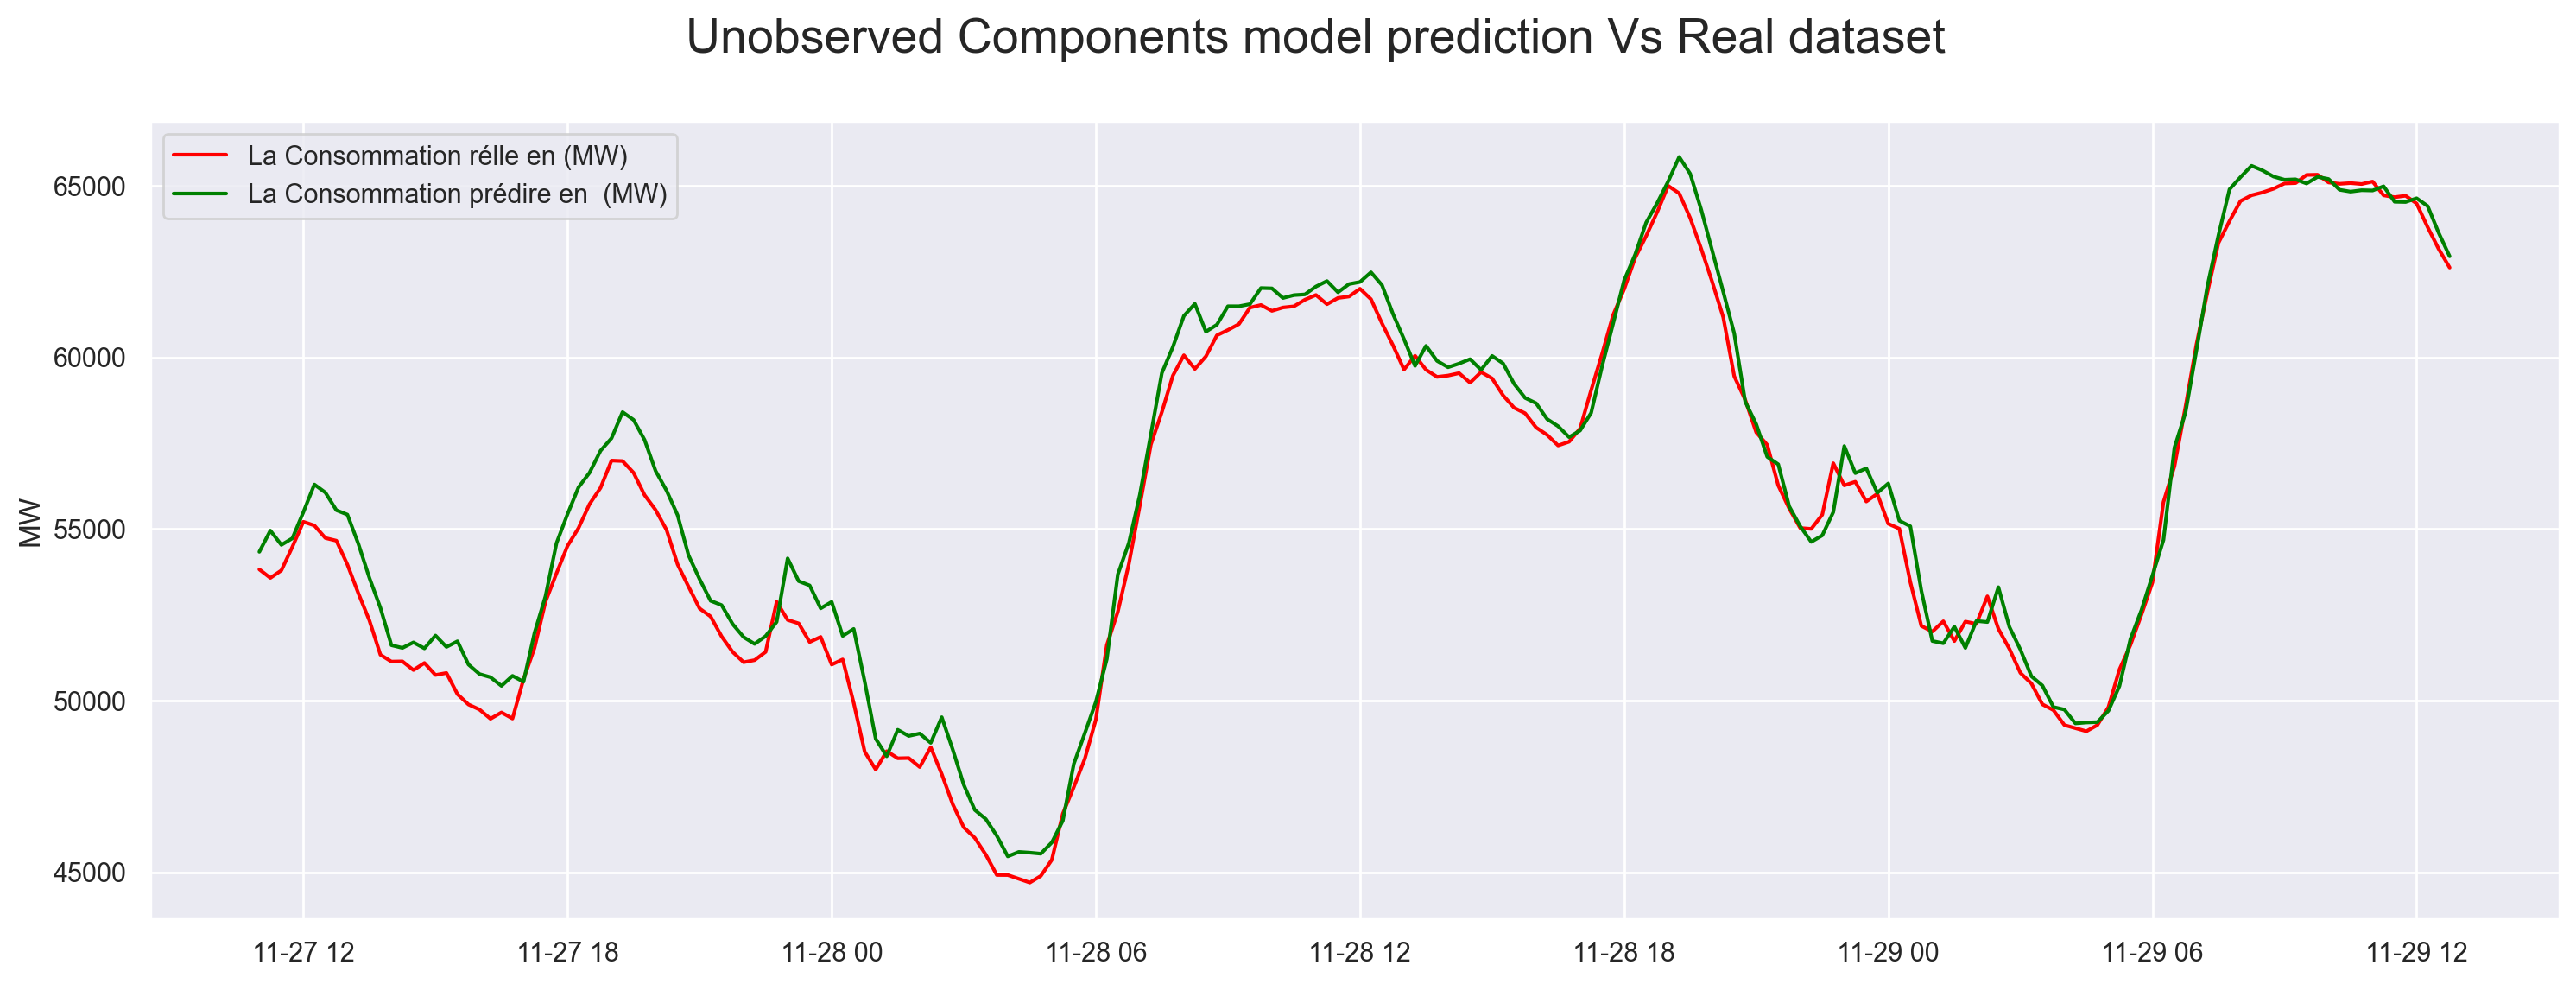
\includegraphics[scale=0.30]{images/outputVV.png}

\end{frame}
%---------------------------------------------------------

\end{document}